\documentclass[18 pt]{beamer}
\usetheme{Madrid}
% \usefonttheme{professionalfonts}
\usefonttheme{structurebold}
\usecolortheme{rose}
\setbeamerfont{title}{size=\LARGE, series=\bfseries}
% \setbeamerfont{subtitle}{size=\large}
% \setbeamerfont{author}{size=\large}
% \setbeamerfont{date}{size=\large}
% \setbeamerfont{frametitle}{size=\Large, series=\bfseries}
% \setbeamerfont{framesubtitle}{size=\large}
% \setbeamerfont{normal text}{size=\huge}
\usepackage{enumitem}
\setlist[enumerate]{label=\arabic*)., leftmargin=*,itemsep=30pt}
\setbeamerfont{enumerate item}{size=\LARGE}
\setlist[itemize]{label=\textbullet, leftmargin=*, itemsep=5pt}

\usepackage{hyperref}
\hypersetup{colorlinks=true, linkcolor=blue, urlcolor=green}
\usepackage{tikz}
\usepackage{braket}
\usepackage{yquant}

\usepackage{amsmath}
\usepackage{amssymb}
\usepackage{listings}
\usepackage{booktabs}
\usepackage{multirow}
\usepackage{multirow}
\usepackage{lmodern}
\usepackage{xcolor}
\usepackage{float}
\lstset{
  language=Python,  %代码语言使用的是matlab
  % frame=shadowbox, %把代码用带有阴影的框圈起来
  rulesepcolor=\color{red!20!green!20!blue!20},%代码块边框为淡青色
  keywordstyle=\color{blue!90}\bfseries, %代码关键字的颜色为蓝色,粗体
  commentstyle=\color{red!10!green!70}\textit,    % 设置代码注释的颜色
  basicstyle=\footnotesize,
  showstringspaces=true,%不显示代码字符串中间的空格标记
  % numbers=left, % 显示行号
  % numberstyle=8pt,    % 行号字体
  % numberstyle=\color{green},
  stringstyle=\rmfamily\slshape\color[RGB]{128,0,0}, % 代码字符串的特殊格式
  breaklines=true, %对过长的代码自动换行
  extendedchars=false,  %解决代码跨页时,章节标题,页眉等汉字不显示的问题
  escapeinside=``,%代码中出现中文必须加上,否则报错
  texcl=true}

\lstset{breaklines}%自动将长的代码行换行排版

\lstset{extendedchars=false}%解决代码跨页时,章节标题,页眉等汉字不显示的问题

\usepackage{textcomp}
% \usepackage[margin=1in]{geometry}
\usepackage{pythonhighlight}
% \usepackage{minted}
\usepackage[backend=bibtex]{biblatex}
%\usepackage[style=authortitle,backend=biber]{biblatex}
\addbibresource{ResearchRabbit_Export_2022_10_20.bib}

\usepackage{algorithm}
\usepackage{algorithmic}
\renewcommand{\algorithmicrequire}{\textbf{Input:}}
\renewcommand{\algorithmicensure}{\textbf{Output:}}

\AtBeginSection[]{
  \begin{frame}
  \frametitle{Outline}
  \tableofcontents[currentsection,hideallsubsections]
  \end{frame}
}
\AtBeginSubsection[]{
  \begin{frame}
  \frametitle{Outline}
  \tableofcontents[currentsubsection]
  \end{frame}
}
\setbeamertemplate{section in toc}{\inserttocsectionnumber.~\inserttocsection}
\setbeamertemplate{subsection in toc}[ball unnumbered]
\setbeamertemplate{subsubsection in toc}[square unnumbered]


\title{Synthesis on Atom Computation}
\author[Gcc]{Dingchao Gao}
\institute[ISCAS]{Institute of Software Chinese Academy of Sciences}

\setbeamertemplate{footline}[frame number]
\begin{document}
\begin{frame}[plain]
    \titlepage
  \end{frame}
% \begin{frame}
%     \frametitle{Outline}
%     \begin{itemize}
%         \item Quick review
%         \item Paper call back
%         \item Discussion
%     \end{itemize}
% \end{frame}

\begin{frame}
    \frametitle{Quick Review of Atom Computation}
    \begin{itemize}
        \item \textbf{Control Mechanisms:} 
            \begin{itemize}
                \item Neutral atoms controlled by laser lattice (stationary) 
                \item Laser tweezers (for movement)
            \end{itemize}
        \item \textbf{Single Qubit Gate:} 
            \begin{itemize}
                \item $U3: (\Omega\tau\cos{\varphi}, \Omega\tau\sin{\varphi}, \delta\tau)$
            \end{itemize}
        \item \textbf{Multi-Qubit Gate:} 
            \begin{itemize}
                \item $C\mathcal{Z}: 2|gg\rangle\langle gg| - I$
            \end{itemize}
    \end{itemize}
\end{frame}

% \begin{frame}
%     \frametitle{Introducing the Paper}
%     \begin{itemize}
%         \item \textbf{Setup:} Key constraints and considerations
%         \item \textbf{Objective:} Cost reduction goals
%         \item \textbf{Methods:} Approach and techniques used
%     \end{itemize}
% \end{frame}

\section{Decomposing and Routing Quantum Circuits Under Constraints for Neutral Atom Architectures}

% \begin{frame}
%     \frametitle{Setup}
%     \begin{itemize}
%         \item \textit{StandardGateSet}: $\{U_3,CZ\}$
%         \item Existing hardware does not support local addressing for all qubit rotations:
%         \begin{itemize}
%             \item Local $CZ$
%             \item Local $R_Z(\lambda), (0,0,\frac{\lambda}{2})$
%             \item Global $GR(\theta,\phi), (\frac{\theta}{2}\cos{\phi},\frac{\theta}{2}\sin{\phi},0)$
%         \end{itemize}
%         \item Atom movement
%     \end{itemize}
% \end{frame}

% \begin{frame}
%     \frametitle{Optimization Goal}
%     The primary optimization goal is to minimize:
%     \begin{itemize}
%         \item Circuit duration 
%         % increase overall fidelity using atom movement for better routing efficiency %
%     \end{itemize}
% \end{frame}
\subsection{Decomposition Strategy}
\begin{frame}
    \frametitle{Decomposition Strategy}
    \begin{itemize}
        \item \textbf{Native Gate Set}
        \begin{itemize}
            \item Local CZ gates.
            \item Local $R_z(\lambda): (0,0,\frac{\lambda}{2})$ gates.
            \item Global $GR(\theta, \phi):(\frac{\theta}{2}\cos{\phi},\frac{\theta}{2}\sin{\phi},0)$ gates.
        \end{itemize}
        \item \textbf{Euler-Angle Decomposition}
        \begin{itemize}
            \item Decompose any single-qubit gate $U3(\theta, \phi, \lambda)$ into Euler angles:
            \[
            U3(\theta, \phi, \lambda) = R_z(\phi) R_y(\theta) R_z(\lambda)
            \]
        \end{itemize}
    \end{itemize}
\end{frame}

\begin{frame}
    \frametitle{Axial Decomposition}
    \begin{itemize}
        \item \textbf{Decomposition of $R_y$ Gate}
        \begin{itemize}
            \item Decompose $R_y(\theta)$ gate into global and local gates:
            \[
            \prod_j R_{y_j}(\theta_j) = GR\left(-\frac{\pi}{2}, 0\right) \left[\prod_j R_{z_j}(\theta_j)\right] GR\left(\frac{\pi}{2}, 0\right)
            \]
            \item This involves a net global rotation of $\pi$.
        \end{itemize}
    \end{itemize}
    \begin{center}
        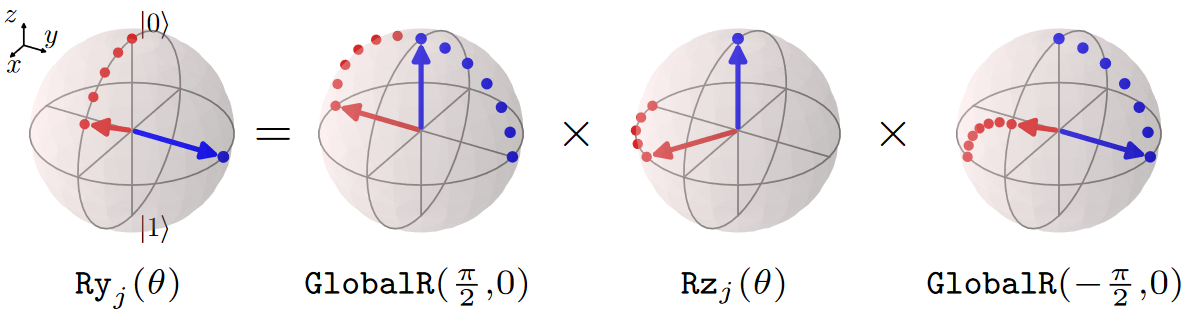
\includegraphics[width=0.9\textwidth]{axial_.png}
    \end{center}
\end{frame}

\begin{frame}
    \frametitle{Transverse Decomposition}
    \begin{itemize}
        \item \textbf{Optimized Decomposition of $R_y$ Gate}
        \begin{itemize}
            \item Decompose $R_y(\theta)$ gate using minimal global rotation angle:
            \[
            R_y(\theta) = R_v\left(\pi, \frac{\theta}{2}\right) R_z(-\pi)
            \]
            \item Further decompose $R_v$ gate into global and local gates:
            \[
            R_v(\xi, \omega) = GR(\omega, \frac{\pi}{2}) R_z(\xi) GR(-\omega, \frac{\pi}{2})
            \]
        \end{itemize}
    \end{itemize}
    \begin{center}
        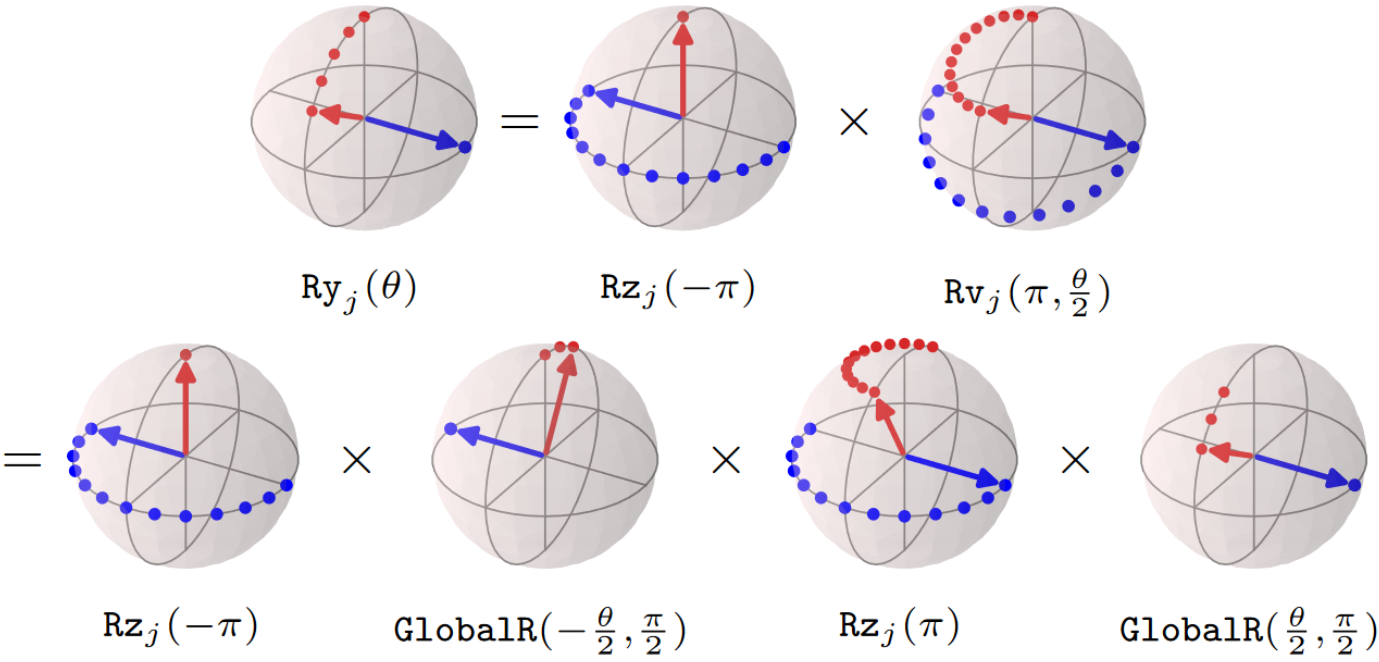
\includegraphics[width=0.8\textwidth]{transverse_.png}
    \end{center}
\end{frame}
\begin{frame}
    \frametitle{Addition step: Post-Processing and Optimizations}
    \begin{itemize}
        \item \textbf{Axis of Rotation Adjustment}
        \begin{itemize}
            \item Change the axis of rotation of global gates to eliminate redundant $R_z$ gates.
        \end{itemize}
        \item \textbf{Gate Merging}
        \begin{itemize}
            \item Merge consecutive $R_z$ gates to further reduce the gate count.
        \end{itemize}
    \end{itemize}
    \begin{center}
        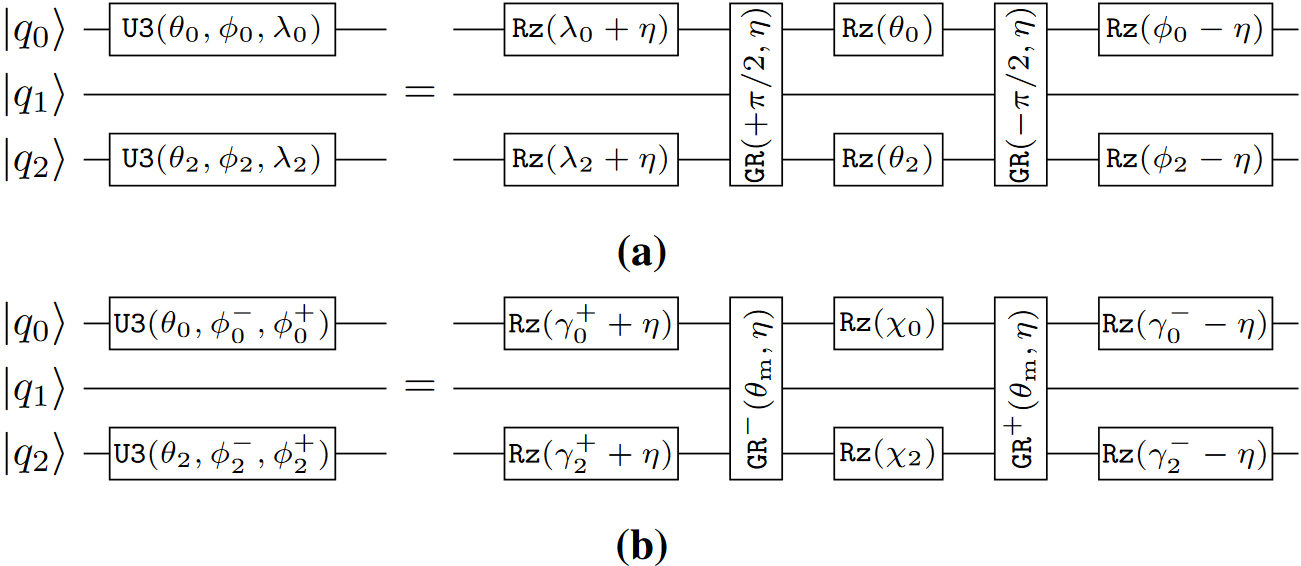
\includegraphics[width=0.8\textwidth]{axis.png}
    \end{center}
\end{frame}
\begin{frame}
    \frametitle{Comparison of Decomposition Methods}
    \begin{itemize}
        \item \textbf{Axial vs. Transverse Decomposition}
        \begin{itemize}
            \item Axial decomposition results in a net global rotation of $\pi$.
            \item Transverse decomposition minimizes global rotation angle to $|\theta|$.
        \end{itemize}
        \item \textbf{Advantages of Transverse Decomposition}
        \begin{itemize}
            \item Up to 3.5x reduction in global gate pulse duration.
            \item Up to 2.9x reduction in single-qubit gate execution time.
        \end{itemize}
    \end{itemize}
\end{frame}

\begin{frame}
    \frametitle{Summary}
    \begin{itemize}
        \item Efficient decomposition of quantum circuits into native gate sets for neutral atom hardware.
        \item Transverse decomposition minimizes global rotation angles, leading to significant speedup.
        \item Post-processing optimizations further reduce gate count and improve execution time.
    \end{itemize}
\end{frame}
% \begin{frame}
%     \frametitle{Methods, \textbf{Decomposition Techniques}}
%     $U3(\theta,\phi,\lambda)= RZ(\phi)RY(\theta)RZ(\lambda)$:
%     \begin{itemize}
%         \item $RY(\theta)= GR(\frac{-\pi}{2},0)RZ(\theta)GR(\frac{\pi}{2},0)$
%         \item $RY(\theta) = Rv(\pi,\frac{\theta}{2})RZ(-\pi)$
%         \item $Rv(\xi,\omega)=GR(\omega,\frac{\pi}{2})RZ(\xi)GR(-\omega,\frac{\pi}{2})$
%     \end{itemize}
% \end{frame}
\subsection{Atom Movement Strategy}
\begin{frame}
    \frametitle{Introduction to Atom Movement}
    \begin{itemize}
        \item \textbf{Goal}
        \begin{itemize}
            \item Utilize physical atom movement to optimize routing in quantum circuits.
            \item Reduce overhead costs associated with traditional SWAP gate decompositions.
        \end{itemize}
        \item \textbf{Challenges}
        \begin{itemize}
            \item Maintain atom fidelity and avoid interference.
            \item Optimize the movement paths to minimize execution time.
        \end{itemize}
    \end{itemize}
\end{frame}

\begin{frame}
    \frametitle{Atom Movement Constraints}
    \begin{itemize}
        \item \textbf{Threshold Distance}
        \begin{itemize}
            \item When moving, an atom must stay at least $d_{\text{thr}}$ away from any other atom to avoid interference.
        \end{itemize}
        \item \textbf{Parallel Movement Constraints}
        \begin{itemize}
            \item Atoms with the same initial $x$-coordinate can move horizontally together only if they end up with the same final $x$-coordinate.
            \item Atoms with the same initial $y$-coordinate can move vertically together only if they end up with the same final $y$-coordinate.
        \end{itemize}
        \item \textbf{Movement Speed}
        \begin{itemize}
            \item Atoms must be moved at speeds not exceeding \textbf{0.55 µm/µs} to maintain qubit fidelity and entanglement.
        \end{itemize}
    \end{itemize}
\end{frame}

\begin{frame}
    \frametitle{Atom Array Configuration}
    \begin{itemize}
        \item \textbf{Initial Mapping}
        \begin{itemize}
            \item Each program qubit is assigned to a unique hardware qubit to minimize routing operations.
        \end{itemize}
        \item \textbf{Displacement}
        \begin{itemize}
            \item Atoms can be displaced from grid points by $d_{\text{thr}}$ to facilitate SWAP operations without violating distance constraints.
        \end{itemize}
    \end{itemize}
    % \begin{center}
    %     \includegraphics[width=0.6\textwidth]{atom_array_configuration.png}
    % \end{center}
\end{frame}

\begin{frame}
    \frametitle{Movement Graph}
    \begin{itemize}
        \item \textbf{Graph Definition}
        \begin{itemize}
            \item Nodes represent atom sites.
            \item Edges indicate direct movement paths between sites without violating $d_{\text{thr}}$.
            \item Edge weights represent the distance between atom sites.
        \end{itemize}
    \end{itemize}
    \begin{center}
        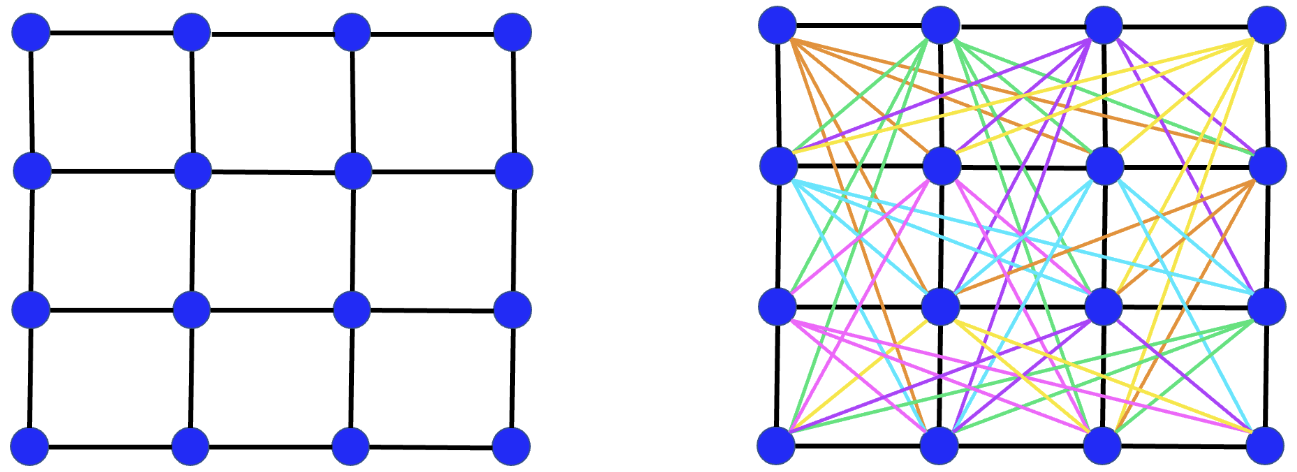
\includegraphics[width=0.6\textwidth]{move.png}
    \end{center}
\end{frame}
\begin{frame}
    \frametitle{CZ Gate Execution Work Flow}
    \begin{itemize}
        % \item \textbf{:}
        \item Use movement graph to determine qubit permutation when a CZ gate $(qa, qb)$ can not be executed with current mapping.
        \item Consider all program qubit pairs $(u, v)$ that:
        \begin{itemize}
            \item $u\in\{qa,ab\}$ or $v\in\{qa,ab\}$.
            \item Have an edge \((m_{t-1}(u), m_{t-1}(v))\) in the movement graph.
            \item Bring $qa$ and $qb$ closer after moving $u$ to $m_{t-1}(v)$ or move $v$ to $m_{t-1}(u)$.
        \end{itemize}
        \item Choose pair $(u', v')$ minimizing distance between $qa$ and $qb$ after permutation.
    % \item \textbf{Execution Logic:}
    % \begin{itemize}
    %     \item Connectivity graph still determines CZ gate execution feasibility.
    %     \item Aim to reduce total operations and movement distance.
    %     \item Minimize disruptions to other qubit mappings.
    % \end{itemize}
    \end{itemize}
\end{frame}
% \begin{frame}
%     \frametitle{Movement Costs and Optimization}
%     \begin{itemize}
%         \item \textbf{Movement Costs}
%         \begin{itemize}
%             \item \textbf{Duration}
%             \begin{itemize}
%                 \item Movement duration is the distance traveled divided by movement speed.
%             \end{itemize}
%             \item \textbf{Errors}
%             \begin{itemize}
%                 \item Atom movements incur idle errors but not gate errors.
%             \end{itemize}
%             \item \textbf{Parallelism}
%             \begin{itemize}
%                 \item Maximize parallel movements while adhering to constraints to optimize circuit duration.
%             \end{itemize}
%         \end{itemize}
%         \item \textbf{Optimization Strategy}
%         \begin{itemize}
%             \item Use movement graph to determine the best paths for atom movement.
%             \item Adjust initial displacements to facilitate efficient SWAP operations.
%         \end{itemize}
%     \end{itemize}
% \end{frame}

\begin{frame}
    \frametitle{Comparing SWAP-based and Movement-based Routing}
    \begin{itemize}
        \item \textbf{SWAP-based Routing}
        \begin{itemize}
            \item SWAP gate decomposition results in high gate count and execution time.
        \end{itemize}
        \item \textbf{Movement-based Routing}
        \begin{itemize}
            \item Atom movement reduces routing overhead and improves fidelity.
            \item Achieves up to 10x speedup and 2x improvement in fidelity.
        \end{itemize}
    \end{itemize}
    % \begin{center}
    %     \includegraphics[width=0.6\textwidth]{routing_comparison.png}
    % \end{center}
\end{frame}

\begin{frame}
    \frametitle{Summary}
    \begin{itemize}
        \item Utilize physical atom movement to optimize routing in neutral atom quantum computers.
        \item Maintain fidelity and avoid interference with strategic movement constraints and optimizations.
        \item Significant improvements in execution speed and circuit fidelity compared to traditional SWAP-based routing.
    \end{itemize}
\end{frame}
% \begin{frame}
%     \frametitle{Compiling Quantum Circuits for Dynamically Field-Programmable Neutral Atoms Array Processors}
% \end{frame}

% \begin{frame}
%     \frametitle{FPQA-C: A Compilation Framework for Field Programmable Qubit Array}
% \end{frame}
\section{Compiling Quantum Circuits for Dynamically Field-Programmable Neutral Atoms Array Processors\\FPQA-C: A Compilation Framework for Field Programmable Qubit Array}
\begin{frame}
    \frametitle{DPQA/FPQA Architecture}
    \begin{itemize}
        \item \textbf{Qubit Traps}
        \begin{itemize}
            \item Qubits are held in optical traps generated by Acousto-Optic Deflectors (AODs) and Spatial Light Modulators (SLMs).
        \end{itemize}
        \item \textbf{Reconfigurability}
        \begin{itemize}
            \item AOD traps can move in rows and columns, allowing dynamic reconfiguration.
            \item AOD rows/columns cannot cross over or overlap during movement.
        \end{itemize}
        \item \textbf{Entangling Gates}
        \begin{itemize}
            \item Entangling gates are applied using a Rydberg laser, effective when qubits are within a blockade range \( r_b \).
        \end{itemize}
    \end{itemize}
\end{frame}
\subsection{Tan}
\begin{frame}
    \frametitle{Overview of the Method}
    \begin{itemize}
        \item \textbf{Goal}
        \begin{itemize}
            \item Develop a compiler for Dynamically Field-Programmable Qubit Arrays (DPQA).
            \item Optimize the placement and routing of qubits to minimize circuit depth.
        \end{itemize}
        \item \textbf{Approach}
        \begin{itemize}
            \item Discretize the state space and formulate the problem as a Satisfiability Modulo Theories (SMT) problem.
            \item Use an SMT solver to find optimal solutions.
        \end{itemize}
    \end{itemize}
\end{frame}
\begin{frame}
    \frametitle{Discretization of State Space}
    \begin{itemize}
        \item \textbf{Space Domain}
        \begin{itemize}
            \item Discretized into interaction sites to ensure qubits are either paired for gates or idle and well-separated.
        \end{itemize}
        \item \textbf{Time Domain}
        \begin{itemize}
            \item Discretized into stages where qubit positions are adjusted and gates are executed.
        \end{itemize}
    \end{itemize}
    % \begin{center}
    %     \includegraphics[width=0.6\textwidth]{discretization.png}
    % \end{center}
\end{frame}
% //TODO: add more constraints, aslso complex analyse
\begin{frame}
    \frametitle{SMT Model Variables}
    \begin{itemize}
        \item \textbf{stage \( s \)}: Represents the stage or step in the quantum circuit execution process.
        \item \textbf{qubit \( q_i \)}: Denotes the \( i \)-th qubit in the quantum circuit.
        \item \textbf{gate \( g_j \)}: Represents the \( j \)-th gate in the quantum circuit.
        \item \textbf{site indices \( x_{i,s}, y_{i,s} \)}: Coordinates \( (x, y) \) of the \( i \)-th qubit at stage \( s \).
        \item \textbf{array index \( a_{i,s} \)}: Indicates whether the \( i \)-th qubit at stage \( s \) is in a stationary SLM trap (\( a_{i,s} = 0 \)) or in a mobile AOD trap (\( a_{i,s} = 1 \)).
        \item \textbf{AOD indices \( c_{i,s}, r_{i,s} \)}: Column \( c \) and row \( r \) indices for the \( i \)-th qubit at stage \( s \) in the AOD grid.
        \item \textbf{time coordinate \( t_j \)}: The time coordinate when the \( j \)-th gate is applied.
    \end{itemize}
\end{frame}

\begin{frame}
    \frametitle{SMT Model Constraints}
    \begin{itemize}
        \item \textbf{Spatial Constraints}
        \begin{itemize}
            \item Qubits must be within the defined grid bounds:
            \[
            0 \leq x_{i,s} < X, \quad 0 \leq y_{i,s} < Y \quad \forall i\in \left[0,N \right), s \in \left[0,S\right)
            \]
            \item AOD moves:
            \[(a_{i,s}=1)\implies (c_{i,s+1}=c_{i,s}\land r_{i,s+1}=r_{i,s})\]
            \item Site order implying row/column order enforing:
            \[(x_{i,s}<x_{i',s})\implies (c_{i,s}<c_{i',s}),\quad (y_{i,s}<y_{i',s})\implies (r_{i,s}<r_{i',s})
            \] 
            \item AOD rows/columns cannot cross each other:
            \begin{small}
                \begin{align*}
                &((a_{i,s} = 1) \land (a_{i',s} = 1) \land (c_{i,s} < c_{i',s})) \implies (x_{i,s+1} \leq x_{i',s+1}), \\
                &((a_{i,s} = 1) \land (a_{i',s} = 1) \land (r_{i,s} < r_{i',s})) \implies (y_{i,s+1} \leq y_{i',s+1}).
                \end{align*}
            \end{small}
        \end{itemize}
    \end{itemize}
\end{frame}
\begin{frame}
    \frametitle{SMT Model Constraints}
    \begin{itemize}
        \item \textbf{Interaction Constraints}
        \begin{itemize}
            \item Qubits must be within \( r_b \) for entangling gates:
            \begin{small}
                \begin{align*}
                    &((a_{i,s-1} = 1) \land (a_{i',s-1} = 1) \land (c_{i,s-1} - c_{i',s-1} \geq C_{\text{STK}})) \implies (x_{i,s} > x_{i',s}), \\
                    &((a_{i,s-1} = 1) \land (a_{i',s-1} = 1) \land (r_{i,s-1} - r_{i',s-1} \geq R_{\text{STK}})) \implies (y_{i,s} > y_{i',s}).
                \end{align*}
            \end{small}
        \end{itemize}
        \item \textbf{Circuit-Dependent Constraints}
        \begin{itemize}
            \item Connectivity ensures:
            \[
                (t_j=s)\implies (x_{i,s}=x_{i',s}\land y_{i,s}=y_{i',s})
            \]
        \end{itemize}
    \end{itemize}
    \begin{center}
        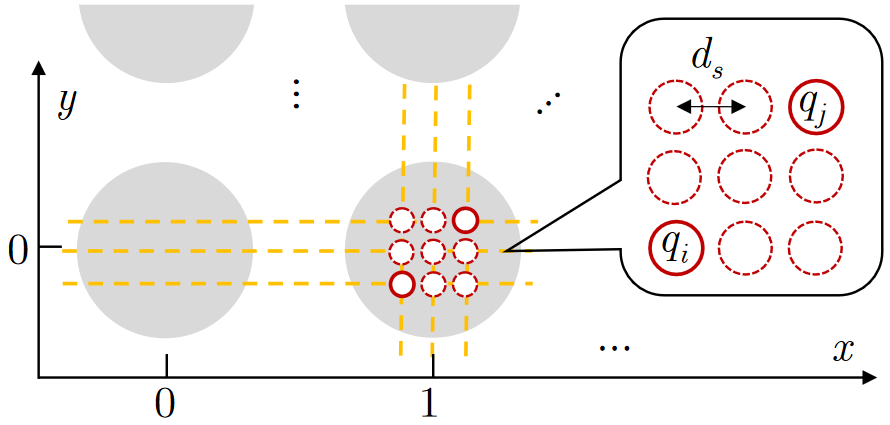
\includegraphics[width=.6\textwidth]{stack.png}
    \end{center}
\end{frame}
\begin{frame}
    \frametitle{Scalability of the Model}
    \begin{itemize}
        \item \textbf{Variables:} \(5NS + G\)
        \item \textbf{Constraints:} \(O(G^2 + GS + N^2S)\)
        \item \textbf{Bits to Represent Variables:} \(NS \log(2XY RC) + G \log(S)\)
        \item \textbf{Worst-Case Runtime:} \(O((N_{SLM}N_{AOD})^{NS }\cdot S ^G)\)
        \item \textbf{Shallow Circuit Regime and sparse graphs (\(G=O(n)\)):}
        \begin{itemize}
            \item Bits required: \(O(N \log(N_{SLM}N_{AOD}))\)
            \item Constraints: \(O(N^2)\)
        \end{itemize}
        % \item \textbf{Hybrid Compiler 'Peeling':} \(S = 2\)
    \end{itemize}
\end{frame}
\begin{frame}
    \frametitle{Example of Compiled Quantum Circuit}
    \begin{center}
        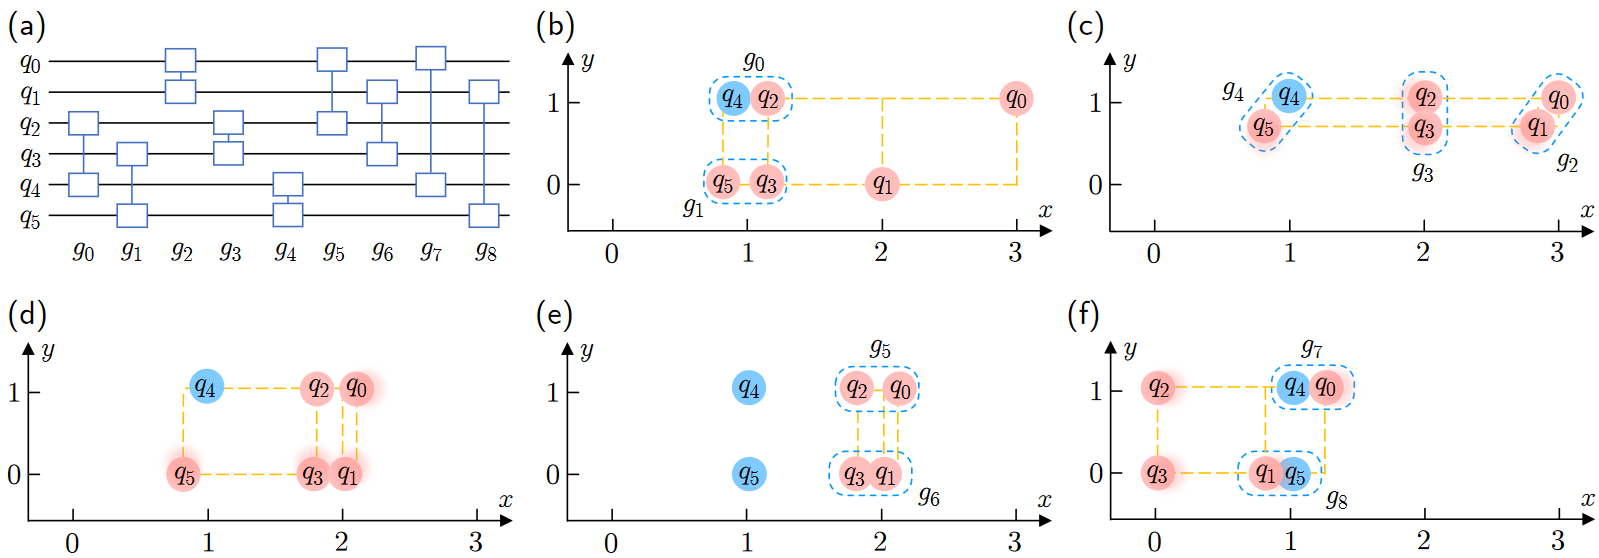
\includegraphics[width=\textwidth]{compile.png}
    \end{center}
\end{frame}
\begin{frame}
    \frametitle{Greedy Heuristic Method}
    \begin{itemize}
        % \item \textbf{Purpose:} Accelerates the compilation for large quantum circuits.
        % \item \textbf{Approach:}
        % \begin{itemize}
        %     \item At each stage, find AOD movements to maximize the number of gates executed in the next stage.
        %     \item Repeat until a small number of gates remain.
        %     \item Switch to the optimal approach for the final stages.
        % \end{itemize}
        % \item \textbf{Inspiration:} Iterative peeling in classical integrated circuit routing.
        \item \textbf{Steps:}
        \begin{itemize}
            \item Construct a "single-step" SMT model with two stages.
            \item Optimize the number of gates executed in the second stage.
            \item Append the solution to the full solution and remove executed gates.
            \item Repeat until fewer than 5\% of gates remain.
        \end{itemize}
        \item \textbf{Benefit:} Significantly faster than the optimal compiler with some sacrifice in optimality.
    \end{itemize}
\end{frame}

% \begin{frame}
%     \frametitle{Hybrid Compilation Approach}
%     \begin{itemize}
%         \item \textbf{Greedy Heuristic}
%         \begin{itemize}
%             \item Iteratively maximize the number of gates executed per stage.
%         \end{itemize}
%         \item \textbf{Optimal Approach}
%         \begin{itemize}
%             \item Use SMT solver to find optimal solutions when problem size is small.
%         \end{itemize}
%     \end{itemize}
%     % \begin{center}
%     %     \includegraphics[width=0.8\textwidth]{hybrid_approach.png}
%     % \end{center}
% \end{frame}
\begin{frame}
    \frametitle{Experimental Results}
    \begin{itemize}
        \item \textbf{Benchmarks:}
        \begin{itemize}
            \item Evaluated on random graphs.
            \item Circuits with 10 to 90 qubits.
        \end{itemize}
        \item \textbf{Main Findings:}
        \begin{itemize}
            % \item DPQA with OLSQ-DPQA compiler reduces two-qubit gates significantly.
            \item For 90-qubit circuits: 5.1x fewer two-qubit gates compared to fixed planar architecture.
        \end{itemize}
        \item \textbf{Error Sources:}
        \begin{itemize}
            % \item Main source: Rydberg laser for two-qubit gates.
            \item AOD movements cause 27x less infidelity.
        \end{itemize}
        \item \textbf{Compiler Performance:}
        \begin{itemize}
            \item Hybrid approach faster than optimal compiler.
            \item Compiles up to 90-qubit circuits within a day.
        \end{itemize}
    \end{itemize}
\end{frame}

\begin{frame}
    \frametitle{Summary}
    \begin{itemize}
        \item Utilize reconfigurability and non-local connectivity of DPQA for efficient quantum circuit compilation.
        \item Formulate constraints as an SMT problem for optimal solutions.
        \item Implement hybrid approach for scalability.
    \end{itemize}
\end{frame}

% \begin{frame}
%     \frametitle{Setup (FPQA)}
%     \begin{itemize}
%         \item Gateset:
%         \begin{itemize}
%             \item Global $CZ$
%             \item Local $U3$
%         \end{itemize}
%         \item Optical traps are configured in 2D arrays.
%         \item Two-qubit entangling gates require qubits to be within a certain proximity without interfering with others.
%         \item Constraints of physical movement of traps, ensuring each solution step complies with the DPQA constraints and remains executable.
%     \end{itemize}
% \end{frame}

% \begin{frame}
%     \frametitle{Constraints in the Greedy Method}
%     \begin{itemize}
%         \item \textbf{DPQA Architectural Constraints}:
%         \begin{itemize}
%             \item Adhere to movement and interaction rules specific to DPQA.
%             \item Maintain the logical sequence of gate operations.
%         \end{itemize}
%         \item \textbf{Minimum Gates Threshold ('M')}:
%         \begin{itemize}
%             \item Strive to achieve at least 'M' gates per stage, where 'M' is dynamically adjusted based on solvability.
%         \end{itemize}
%         \item \textbf{SMT Solver Integration}:
%         \begin{itemize}
%             \item Use an SMT solver to find feasible solutions that maximize gate execution while respecting the constraints.
%         \end{itemize}
%     \end{itemize}
% \end{frame}

% \begin{frame}
%     \frametitle{SMT Solver Role in the Greedy Method}
%     \begin{itemize}
%         \item \textbf{Input}: Reduced and simplified problem instances as the complexity is peeled off.
%         \item \textbf{Output}: Feasible configurations that allow the maximum number of gates ('M') to be executed per stage.
%         \item \textbf{Dynamic Adjustment}: Modifies 'M' based on the ease or difficulty of finding a solution, optimizing the balance between speed and completeness of the solution.
%     \end{itemize}
% \end{frame}

% \begin{frame}
%     \frametitle{Transition to Optimal Compilation}
%     \begin{itemize}
%         \item \textbf{Criterion for Transition}: Shifts to the optimal SMT-based approach when a significant portion of the problem has been resolved or when only a small percentage of gates remains.
%         \item \textbf{Rationale}: Ensures that the final solution is both efficient and adheres strictly to all operational constraints.
%     \end{itemize}
% \end{frame}

% \begin{frame}
%     \frametitle{Conclusion}
%     The integration of the SMT solver within the Greedy Method in this hybrid approach allows for a pragmatic reduction of quantum circuit complexity, setting the stage for a detailed and optimal final compilation using SMT.
% \end{frame}

% \begin{frame}
%     \frametitle{Methods (FPQA)}
%     \begin{itemize}
%         \item Qubit-Array Mapper:
%         \begin{itemize}
%             \item K-cut problem aiming to maximize the summation of edge weights crossing different partitions
%         \end{itemize}
%         \item Qubit-Atom Mapper:
%         \begin{itemize}
%             \item SLM Array: Load balance mapping
%             \item AOD Array: Alignment AOD mapping
%         \end{itemize}
%         \item High-Parallelism Router:
%         \begin{itemize}
%             \item U3 gate
%             \item Check constraint
%         \end{itemize}
%     \end{itemize}
% \end{frame}

\subsection{Wang}
% \begin{frame}
%     \frametitle{Overview of FPQA-C}
%     \begin{itemize}
%         \item \textbf{Goal}
%         \begin{itemize}
%             \item Develop a scalable compilation framework for Field Programmable Qubit Array (FPQA).
%             \item Optimize qubit mapping, atom movement, and gate scheduling to minimize circuit depth and error rates.
%         \end{itemize}
%         \item \textbf{Challenges}
%         \begin{itemize}
%             \item Hardware constraints such as non-overlapping AOD movements and compulsory 2Q gates within the Rydberg range.
%             \item Balancing fidelity and parallelism while adhering to hardware limitations.
%         \end{itemize}
%     \end{itemize}
% \end{frame}

\begin{frame}
    \frametitle{Compilation Framework}
    \begin{itemize}
        \item \textbf{Qubit-Array Mapper}
        \begin{itemize}
            \item Uses MAX k-Cut on a gate frequency graph to minimize SWAP overhead.
            \item Coarse-grained mapping of qubits to arrays.
        \end{itemize}
        \item \textbf{Qubit-Atom Mapper}
        \begin{itemize}
            \item Fine-grained mapping of qubits to specific atoms in the array.
            \item Load balance to prevent hardware constraint violations.
        \end{itemize}
        \item \textbf{High-Parallelism Router}
        \begin{itemize}
            \item Iteratively identifies parallelizable 2Q gates.
            \item Decides atom movements and gate executions to maximize parallelism.
        \end{itemize}
    \end{itemize}
\end{frame}

% \begin{frame}
%     \frametitle{Atom Movement Constraints}
%     \begin{itemize}
%         \item \textbf{Non-Overlapping Movements}
%         \begin{itemize}
            
%         \end{itemize}
%         \item \textbf{Compulsory 2Q Gates}
%         \begin{itemize}
%             \item All atom pairs within the Rydberg range must perform CZ gates together.
%         \end{itemize}
%         \item \textbf{Sequential Constraints}
%         \begin{itemize}
%             \item Movement schedules must ensure no illegal row/column swaps.
%         \end{itemize}
%     \end{itemize}
% \end{frame}

\begin{frame}
    \frametitle{Qubit-Array Mapping Method}
    \begin{itemize}
        \item \textbf{MAX k-Cut}
        \begin{itemize}
            \item Finds mapping that maximizes inter-array 2Q gates.
            \item Greedy algorithm used for approximation.
        \end{itemize}
        \item \textbf{Gate Frequency Graph}
        \begin{itemize}
            \item Vertices represent qubits, edges represent gates.
            \item Edge weights determined by gate frequency.
        \end{itemize}
    \end{itemize}
    \begin{center}
        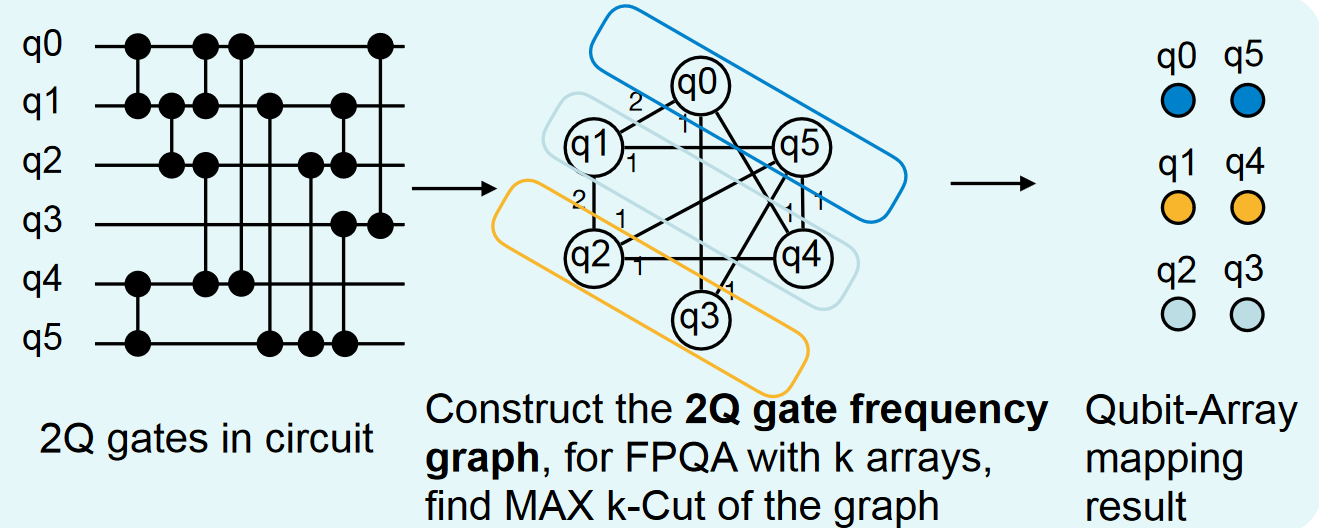
\includegraphics[width=0.6\textwidth]{max_cut.png}
    \end{center}
\end{frame}

\begin{frame}
    \frametitle{Qubit-Atom Mapping Method}
    \begin{itemize}
        \item \textbf{Load Balance Mapping}
        \begin{itemize}
            \item Ensures balanced distribution of qubits across rows and columns.
            \item Avoids constraint violations from dense qubit clusters.
        \end{itemize}
        \item \textbf{Alignment Mapping}
        \begin{itemize}
            \item Maps qubit pairs with frequent 2Q gates to the same positions in different arrays.
            \item Enhances parallelism by aligning high-frequency gates.
        \end{itemize}
    \end{itemize}
    \begin{center}
        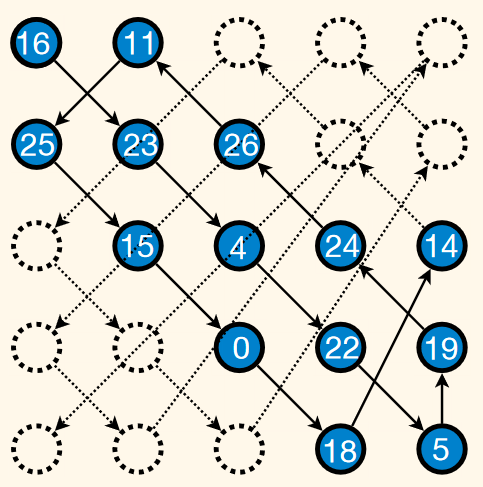
\includegraphics[width=0.3\textwidth]{load.png}
    \end{center}
\end{frame}

\begin{frame}
    \frametitle{High-Parallelism Router}
    \begin{itemize}
        \item \textbf{Non-Dependent Frontier Gates}
        \begin{itemize}
            \item Identifies and schedules gates with no dependencies.
        \end{itemize}
        \item \textbf{Constraint Checks}
        \begin{itemize}
            \item Ensures movements do not violate spatial or interaction constraints.
            \item Greedily adds gates to the parallel set, checking each for legality.
        \end{itemize}
    \end{itemize}
    % \begin{center}
    %     \includegraphics[width=0.6\textwidth]{router_pipeline.png}
    % \end{center}
\end{frame}

% \begin{frame}
%     \frametitle{Experimental Setup}
%     \begin{itemize}
%         \item \textbf{Benchmarks}
%         \begin{itemize}
%             \item Diverse set of benchmarks including QASMBench, SupermarQ, Quantum Simulation, and QAOA circuits.
%         \end{itemize}
%         \item \textbf{Metrics}
%         \begin{itemize}
%             \item 2Q gate count, circuit depth, and fidelity.
%             \item Comparisons with IBM superconducting, FAA with long-range gates, and other topologies.
%         \end{itemize}
%     \end{itemize}
% \end{frame}

\begin{frame}
    \frametitle{Unique Experimental Approach}
    \begin{itemize}
        \item \textbf{Comprehensive Simulations}
        \begin{itemize}
            \item Evaluates logical error rates, execution times, and physical qubit requirements.
            \item Includes realistic modeling of movement overheads (heating, cooling, decoherence, atom loss).
        \end{itemize}
        \item \textbf{Scalability and Performance}
        \begin{itemize}
            \item Demonstrates significant reductions in 2Q gate count and circuit depth.
            \item Achieves up to 1000x faster compilation speed compared to solver-based methods.
        \end{itemize}
    \end{itemize}
\end{frame}

\begin{frame}
    \frametitle{Summary}
    \begin{itemize}
        \item FPQA-C effectively addresses qubit mapping, atom movement, and gate scheduling in FPQA.
        \item Incorporates innovative methods to handle hardware constraints and optimize performance.
        \item Experimental results highlight the advantages of FPQA-C over traditional approaches in terms of gate count, depth, and fidelity.
    \end{itemize}
\end{frame}
\section{Discussion}
\begin{frame}
    \frametitle{map}
    \begin{figure}
        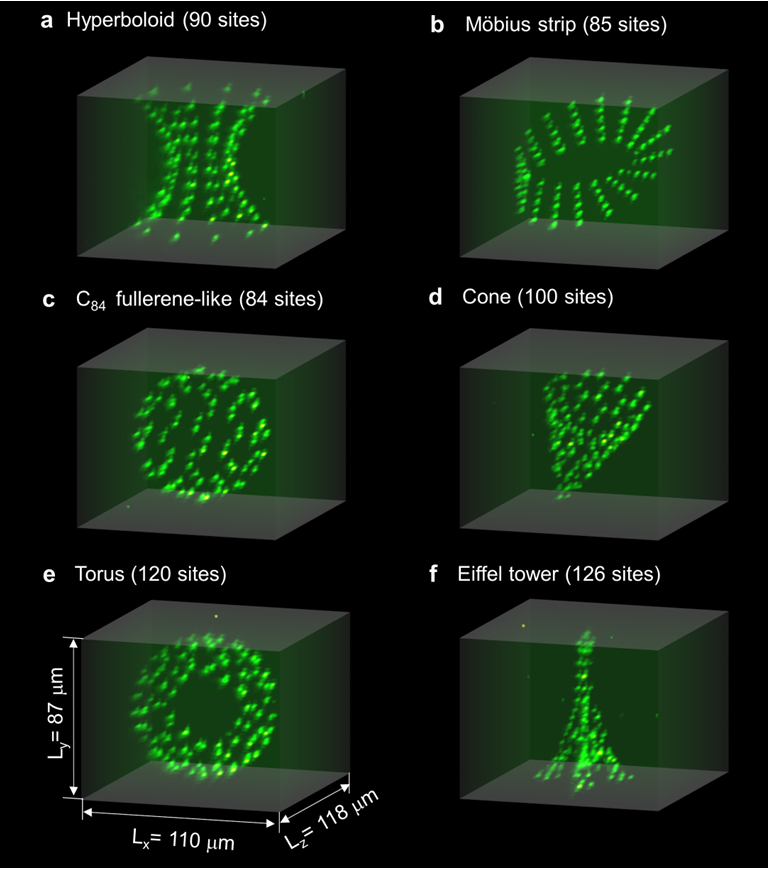
\includegraphics[height = 7cm]{map.png}
        \caption{3D map from \href{https://arxiv.org/abs/1712.02727}{DB17}. Q1: Differences between 2D and 3D mapping.}
    \end{figure}
\end{frame}
\begin{frame}
    \frametitle{CZ ? C$\mathcal{Z}$}
    \begin{columns}
        \begin{column}{.5\textwidth}
            \begin{itemize}
                \item $C\mathcal{Z}: 2|gg\rangle\langle gg| - I$, while $CZ: I - 2|11\rangle\langle 11|$
                \item in gererally:
                \begin{align*}
                    |gg\rangle & \rightarrow |gg\rangle \\
                    |ge\rangle & \rightarrow |ge\rangle e^{i\phi_1} \\
                    |eg\rangle & \rightarrow |eg\rangle e^{i\phi_1} \\
                    |ee\rangle & \rightarrow |ee\rangle e^{i(2\phi_1 + \pi)}
                \end{align*}
            \end{itemize}
        \end{column}
        \begin{column}{.5\textwidth}
            \begin{figure}
                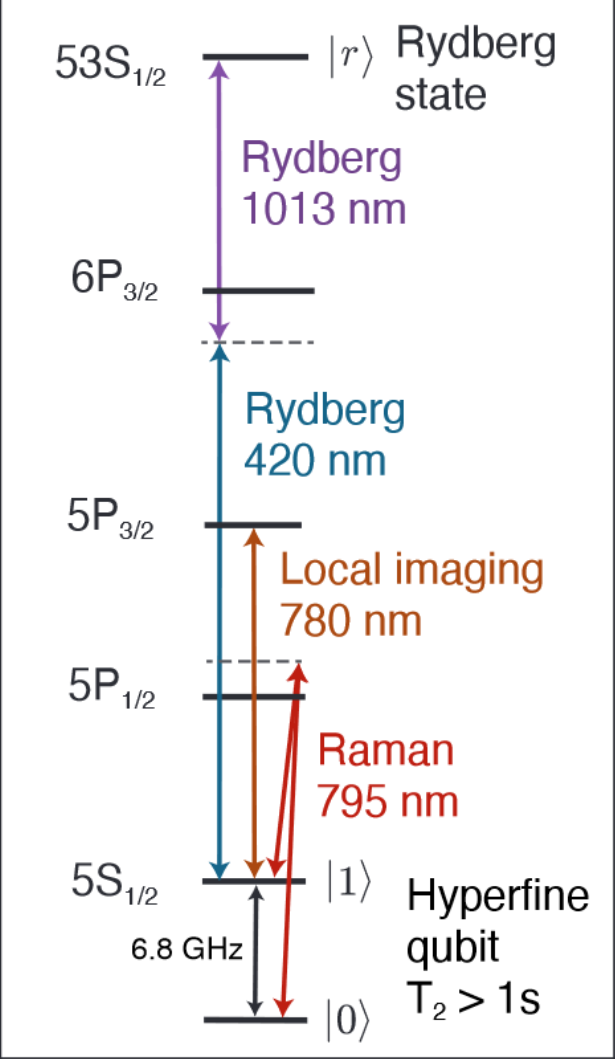
\includegraphics[width=.5\textwidth]{level.png}
                \caption{Level structure for $^{87}Rb$ atoms, with the relevant atomic transitions employed in \href{http://arxiv.org/abs/2312.03982}{\textit{Quera paper}}.}
            \end{figure}
        \end{column}
    \end{columns}
\end{frame}
\begin{frame}
    \frametitle{How to use mcz}
    \begin{figure}
        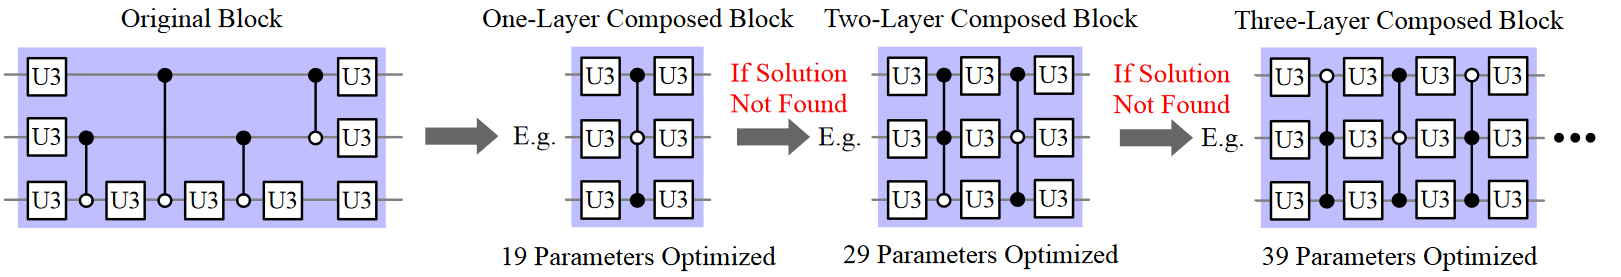
\includegraphics[width=\textwidth]{gyser.png}
        \caption{Main idea in \href{https://dl.acm.org/doi/10.1145/3470496.3527428}{Gyser paper}. Q2: Applying some rules to gap the CZ gate circuit and MCZ gate circuits.
        }
    \end{figure}
\end{frame}
\begin{frame}
    \frametitle{How to use mcz}
    \begin{itemize}
        \item Q3: How to use mcz to construct circuit directly.
    \end{itemize}
    \begin{figure}
        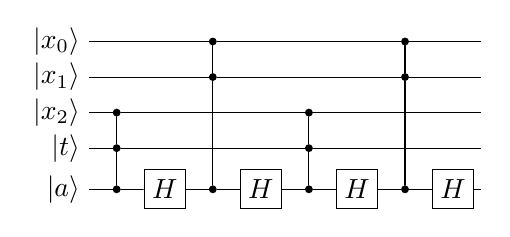
\begin{tikzpicture}
            \begin{yquant*}
                qubit {$\ket{x_\idx}$} q[3];
                qubit {$\ket{t}$} q[+1];
                qubit {$\ket{a}$} q[+1];
                zz (q[2-4]);
                H q[4];
                zz (q[0,1,4]);
                H q[4];
                zz (q[2-4]);
                H q[4];
                zz (q[0,1,4]);
                H q[4];
            \end{yquant*}
        \end{tikzpicture}
            \caption{use ccz and Hadmard gate to construct cccz gate.}
        \end{figure}
\end{frame}

\end{document}
